\documentclass[12pt,journal]{IEEEtran}
\usepackage[T1]{fontenc} % optional
\usepackage{amsmath}
\usepackage[cmintegrals]{newtxmath}
\usepackage{bm} % optional
\usepackage{wrapfig}
\usepackage{graphicx} %package to manage images
\usepackage[utf8]{inputenc}
\usepackage{enumerate}
\usepackage{longtable}
\title{Rank Fusion \\ {\huge Information Retrieval Project}}
\author{Davide Rigoni - Silvia Colucci - Alex Beccaro \\ January 29, 2018}	

\begin{document}
	\maketitle
	%chapters
	%\begin{abstract}

\end{abstract}

	%\section{Conclusion}
\begin{frame}{Conclusion}
	%\begin{enumerate}
	%\end{enumerate}
\end{frame}



	\textbf {Abstract— Recently researches have focused on the idea that performance and the effectiveness of individual IR models can be improved by combining the outputs of some individual models into a single result set. Data fusion is the combination of the results of independent searches on a document collection into one single output result set. In fact, ranking quality can be achieved by adopting different strategies and so different retrieval models.
In this regard, we have implemented some rank fusion base strategies to perform retrieval experiments by generating runs and by comparing their individual results with results obtained by ten runs of different systems through Terrier.
Afterwards, we have implemented an advanced rank fusion strategy called ProbFuse to perform another results comparison and to look for eventual improvements compared to the popular fusion algorithms. We have reported also a ProbFuse variant after the IIX section namely ProbFuse Variant, whose explanations can be found in the VII section namely Implementation Issues.} \\

%introduction
\textbf{I. INTRODUCTION} \\
It has been shown in the past that rank fusion can greatly improve retrieval effectiveness over that of the individual results.
This improvement can be achieved by evaluating the results obtained by implementation of different rank fusion algorithms and by the developing and comparing new rank fusion techniques.
In this work ten runs have been generated through Terrier by choosing different IR models to catch all the important features from the given files collection. Then, we have implemented the following classical rank fusion algorithms: CombSUM, CombMAX, CombMNZ, CombANZ and CombMIN. Through these ones we have assessed the generated runs and compared them with those ones previously obtained through Terrier. 
Finally, we have realized the ProbFuse algorithm described in the reference paper: an interesting method that could led us to the achievement of better IR results.
ProbFuse’s idea consists in ranking documents based on their probability of relevance to the given topic in a certain k segment. This probability depends on the position in which each document is returned in the input result set. 
The inputs to the fusion process are produced by different IR models that use the same topics on the document collection. At the beginning of this implementation we had realized a similar algorithm by considering the variable length of each topic, then we have corrected our initial hypotesis and followed the ProbFuse paper indications. We have reported also this one in the last section.\\

\textbf{II.	COLLECTION FILE UNPACKING} \\
At the beginning it has been difficult to decompress the collection files because it was not clear how they were compressed. The zip file needed one decompression program but it contained other zipped files that needed another decompression program, they were compressed by using Unix. Moreover some file were named with their names followed by an integer number and their extension names, such as if they were divided in small groups, for example there were two files named "FR940707.0Z" and "FR940707.1Z" that seemed to be parts of the same file.
They needed to be renamed, so it has been written a bash file to specify how to rename and decompress them automatically.
 \\

\textbf{III. INDEXING} \\
We used Terrier to index Trec collection. 
We found that Terrier’s 4.2 version was bugged and so we had to use the 4.1 version to index all the files.
At the beginning, it was unknown what was the correct format and the exact markup structure to adopt for the given collection for Terrier, so it has been complicated to understand how to set up the properties file and create the indexing with the appropriate lexical analysis, stop-word removal, stemmer and the other settings. The stop-list and the stemmer used for indexing are those ones of Terrier used for English language, the stemmer is PorterStemmer. \\

\textbf{IV. CHOICE OF IR MODELS FOR RUN GENERATION} \\
The following models have been chosen though Terrier to generate ten runs to evaluate subsequently: 
\begin{enumerate}
\item TFIDF
\item BM25
\item DFRBM25 (DFR)
\item LGD (DFR)
\item PL2 (DFR)
\item InexpC2 (DFR)
\item InL2 (DFR)
\item DLH13 (DFR)
\item IFB2 (DFR)
\item BB2 (DFR)
\end{enumerate}
Runs were generated using models standard parameters.
These are very different models based in sundry approaches, some of them have something in common, other use different functions if we compare them to some others, so they are different each other generally. In this way, the rank fusion should achieve better results, because if it takes values from all the individual models, it can capture collection qualities and strength elements given by these and so the fusion should report better results. \\

\textbf{V. NORMALIZATION} \\
The normalization used in this work has been the Standard Normalization which calculates normalized scores by using the maximum and the minimum scores given in the result set. 
The minimum score is subtracted to the unnormalized score of each run element and then this result is divided for the difference between the maximum score and the minimum score.
After the score normalization, the followed combination functions for the scores combination have been implemented: CombMAX, CombSUM, CombMNZ, CombMIN, CombANZ.
They allow to carry out the rank fusion. \\

\textbf{VI.	PROBE FUSE ALGORITHM} \\
ProbFuse algorithm needs to build a set of probabilities for each input model. 
The analysis of the performance of each individual model on training queries allow to calculate these probabilities. 
To calculate these probabilities we need runs given by the individual models and to divide each topic of each run in k segments. For each segment we count relevant and not relevant documents and we calculate the probability considering each relevant document d returned by query considering each topic. 
So, for each segment we want to calculate the probability that a relevant document returned in this segment is relevant according to the given query. Each probability is obtained by the relationship between the number of documents in segment k that are judged to be relevant to query q and the number of documents in k segment that are judged to be relevant added to those ones that are judged to be non relevant to the query.
\[P(d_k\mid m)=\frac{R_k}{R_k+NR_k}\]
Then, on the various runs it is calculated the sum of the probabilities previously calculated with weight  $\frac{1}{k}$, k indicates the number of segment where it appears.
The final score is the result of the followig sum:
\[s_d=\sum_{m\in M}\frac{P(d_k\mid m)}{k}\]
Thus, the resulting elements will form the fused run by using the probabilities calculated. 
We have considered before twenty segments and subsequently fifty segments, because these ones have produced more satisfying results in ProbFuse paper and we wanted to test with these ones. Subsequently we have tried Probfuse with other k values, in particular: seventy, ninety and hundred and ten segments, because by increasing the number of segments we obtained results improvements. In fact, in assessment phase we have discovered that we can obtain better results by using one hundred and ten segments. We have also implemented another similar approach to ProbFuse. We'll discuss about it in the last section called "ProbFuse variant". \\

\textbf{VII. IMPLEMENTATION ISSUES} \\
At first, it took a lot of time to execute main, the fusion phase was very slow; the slowness was due to the structure used for Standard Rank Fusion functions. This problem has been solved by changing the structure from List to HashMap. 
In these functions the research by score of run elements needed to iterate all run elements list, so complexity was O(n). Instead, by introducing HashMap structure the access for example to the element with maximum score value can occur directly. In this way the complexity is reduced to O(1) and main program can be executed in few minutes. 
During the printing phase on file there was another problem: during this operation, after the execution of for cycle that iterates inside the run, it was created a single string. It took run’s rows and created a single string that was passed to an object which wrote a single string on file, but the string object was immutable and so every time it was created a new object copied by precedent string that added the new row. This caused copy of every run rows. This has been solved by using an object able to write on file through enqueuing elements inside a buffer, so that an element can be enqueued after the previous, the copy is avoided and the problem disappears.
Furthermore, when we have started to implement ProbFuse algorithm we thought we had to consider run's subparts composed by k documents instead to divide each run in k segments, because we thought that the different lengths of the topics could be a problem in the calculation of the probabilities required by ProbFuse algorithm, but evaluating result runs we found out that it was not so good. Then we have fixed algorithm implementation. In the end we have reported both ProbFuse results. 
 \\

\textbf{VIII.	RUN ASSESSMENT} \\
We have used Matters library to assess all the different strategies adopted in this work and so to calculate all the necessary assessment measures and generate some plots.
The principal measures performed for the various comparisons have been: the calculation of precision in different cut-off levels, RPrec, Average Precision and Mean Average Precision (MAP).
Precision has been calculated by considering ten and thirty cut-off levels because for many research tasks it is important to consider results ranking in a certain range, and so to mark runs that have relevant documents in high positions. For this purpose, we have considered ten and thirty cut-off levels according to the tasks needs. We have calculated also precision with cut-off level equal to the recall base (the number of the relevant documents in the pool for a certain topic), that currently is one of the most important measures used for IRs assessment.
Instead, Average Precision is another important measure presently used that gives more power to relevant documents which correspond to high rank.
Finally it has been calculated Mean Average Precision through Average Precision values calculated previously.
By comparing measures between runs evaluated by Terrier and those returned by standard rank fusion implemented algorithms, it has been noticed that on average the measures values of the different strategies are very similar. The comparison between MAP measures that we have reported can confirm this.

\begin{table}[h!]
\centering
\caption{MAP values}
\begin{tabular}{|l|l|l|l|l|}
\hline
ComMNZ & ComMAX & ComSUM & CombANZ & CombMIN \\ \hline
0.1871 & 0.1831 & 0.1874 & 0.1833 & 0.1301 \\ \hline
\end{tabular}
\end{table}

\begin{table}[h!]
\centering
\begin{tabular}{|l|l|l|l|l|l|l|l|l|l|}
\hline
BB2    & BM25   & DFR\_BM25 & TF-IDF & DLH & IFB2     \\ \hline
0.1882 & 0.1828 & 0.1835    & 0.1821 & 0.1830 & 0.1881 \\ \hline

\end{tabular}
\end{table}

\begin{table}[h!]
\centering
\begin{tabular}{|l|l|l|l|l|l|l|l|l|l|}
\hline
InL2   & In\_expC2 & LGD    & PL2        \\ \hline
0.1854 & 0.1826    & 0.1882 & 0.1683      \\ \hline

\end{tabular}
\end{table}


Higher values can be obtained through rank fusion standard methods for some topics, but there are also some lower values for other topics compared to runs generated by Terrier. This difference is very small so it can be considered negligible. We have reported Average Precision plot considering the three best standard rank fusion strategies compared with the best three runs evaluated by Terrier derived from three IR models previously choosen.
\begin{figure*}
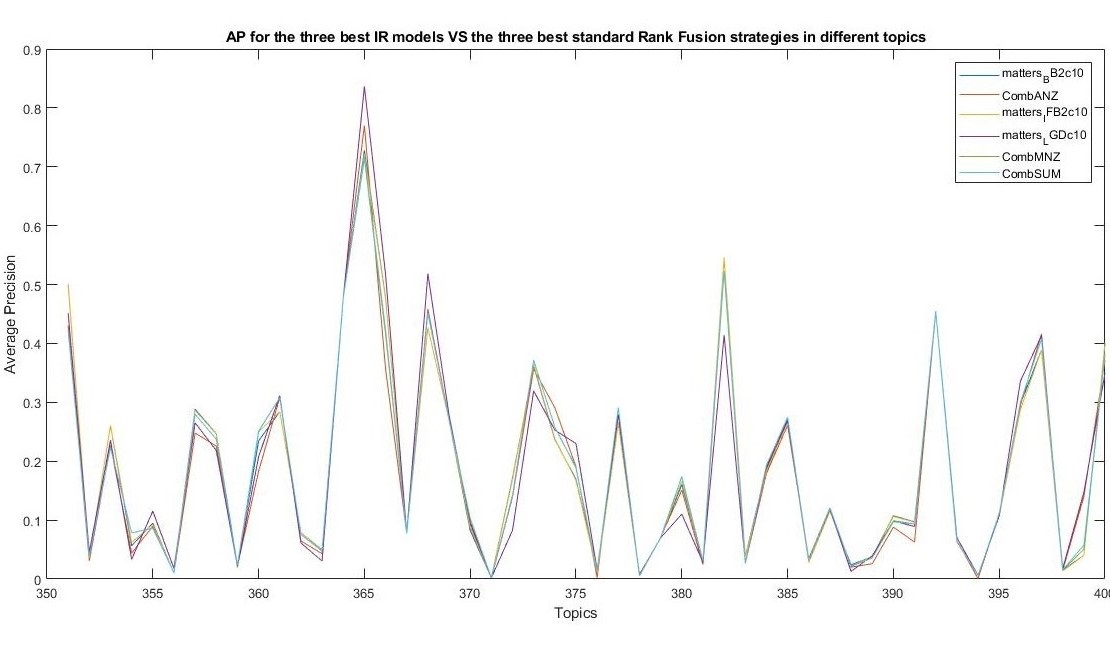
\includegraphics[scale=0.6]{plot1}
\caption{Average Precision for the three best standard Rank Fusion strategies VS the best three IR models in different topics}
\label{Average Precision for the three best standard Rank Fusion strategies VS the best three IR models in different topics}
\end{figure*}

By calculating the assessment measures of rank fusion obtained with ProbFuse we have obtained the best results by considering one hundred and ten segments. \\
The increasing of the number of segments is proportional to the improvement of assessment measures results. This can be noticed by looking the following MAP measures for different ProbFuse k segments reported. 

\begin{figure*}
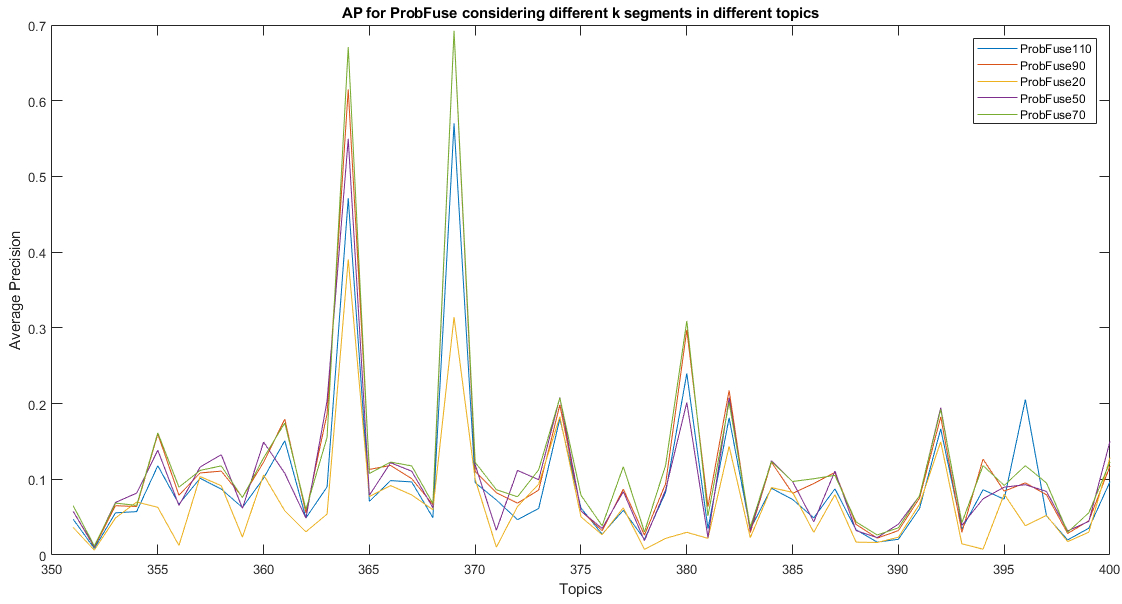
\includegraphics[scale=0.6]{plot4}
\caption{Average Precision for ProbFuse considering different k segments in different topics}
\label{Average Precision for ProbFuse considering different k segments in different topics}
\end{figure*}

\begin{table}[h!]
\centering
\caption{ProbFuse MAP values}
\begin{tabular}{|l|l|l|l|l|}
\hline
k=110 & k=90 & k=70 & k=50 & k=20\\ \hline
 0.1585 & 0.1475 & 0.1260 & 0.1106  & 0.0696\\ \hline
\end{tabular}
\end{table}

Furthermore, we have noticed that all the assessment values obtained through the different measures aren’t very similar with those ones of the standard rank fusion strategies. \\
In the better ProbFuse obtained (considering one hundred and ten segments) we have observed better results for topics from 354 to 356, from 362 to 365, from 368 to 371 and for 380. \\ This can be seen by observing the plot in the Fig.3.

\begin{figure*}
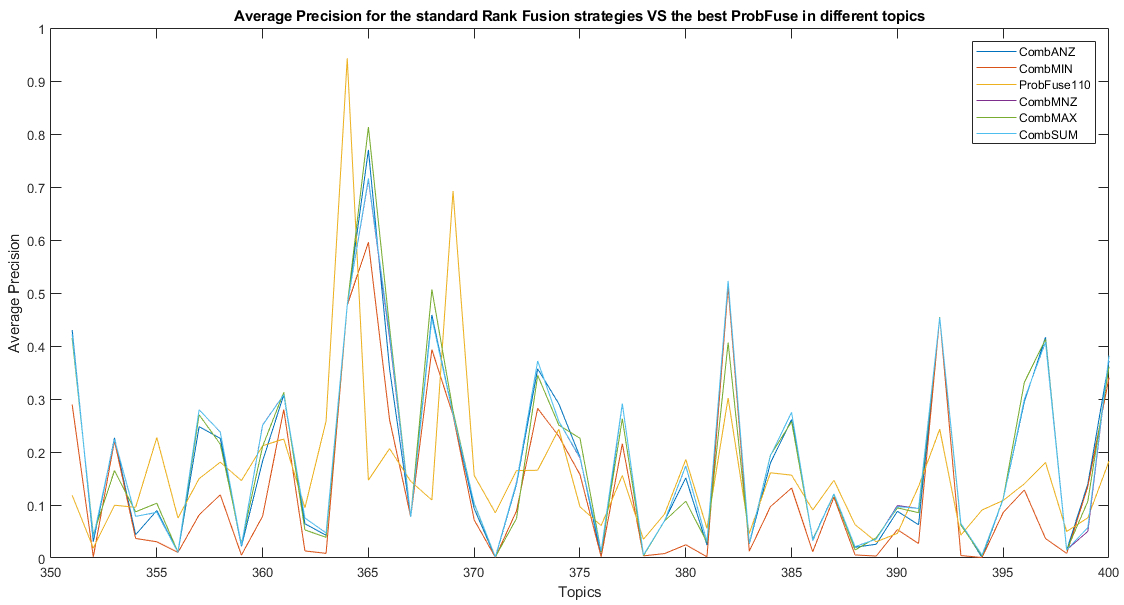
\includegraphics[scale=0.6]{plot2}
\caption{Average Precision for Standard Rank Fusion strategies VS ProbFuse in different topics}
\label{Average Precision for Standard Rank Fusion strategies VS ProbFuse in different topics}
\end{figure*}

We have also reported small examples where ProbFuse results are better than those obtained through standard strategies for different assessment measures in the following tables. \\


\begin{table}[h!]
\centering
\caption{comparison for Average Precision values}
\begin{tabular}{|l|l|l|l|l|}
\hline
T   & ComMNZ    & ComMAX   & ComSUM    & ProbFuse \\ \hline
355 & 0.086124  & 0.10336  & 0.086233  & 0.227280 \\ \hline
363 & 0.047316  & 0.039032 & 0.047187  & 0.258369  \\ \hline
380 & 0.17362   & 0.10718  & 0.17408   & 0.185909  \\ \hline
\end{tabular}
\end{table}

\begin{table}[h!]
\centering
\caption{comparison for Rprec values}
\begin{tabular}{|l|l|l|l|l|}
\hline
T   & ComMNZ   & ComMAX  & ComSUM   & ProbFuse \\ \hline
363 & 0.125    & 0.0625  & 0.125    & 0.25     \\ \hline
387 & 0.1176  & 0.1412 & 0.1176  & 0.1529  \\ \hline
394 & 0.058824 & 0       & 0.058824 & 0.1176  \\  \hline
\end{tabular} 
\end{table}


\begin{table}[h!]
\centering
\caption{comparison for precision values at ten cut-off level}
\begin{tabular}{|l|l|l|l|l|}
\hline
T   & ComMNZ & ComMAX & ComSUM & ProbFuse \\ \hline
363 & 0.2    & 0.1    & 0.2    & 0.3     \\ \hline
369 & 0.3    & 0.3    & 0.3    & 0.9     \\ \hline
374 & 0.4    & 0.4    & 0.4    & 0.7      \\ \hline
\end{tabular}
\end{table}

\begin{table}[h!]
\centering
\caption{comparison for precision values at thirty cut-off level}
\begin{tabular}{|l|l|l|l|l|}
\hline
T   & ComMNZ   & ComMAX   & ComSUM   & ProbFuse \\ \hline
359 & 0.033333 & 0.033333 & 0.033333 & 0.2000  \\ \hline
370 & 0.1      & 0.13333  & 0.1      & 0.3333  \\ \hline
379 & 0.033333 & 0.033333 & 0.033333 & 0.1333     \\ \hline
\end{tabular}
\end{table}

\textbf{IX.	PROBFUSE VARIATION}

In this other ProbFuse implemention we have considered run's subparts of each individual model containing k documents instead to divide runs in k segments. We have considered different sizes for these subparts, in particular we have tested them considering fifteen, twenty, thirty and fifty documents. In the assessment phase we have obtained the best results with subparts of fifteen documents. In general, results obtained by considering all the assessment measures have been lower than original ProbFuse algorithm as can be seen by Fig.4, but for a few specific topics the output results have been even better than those obtained through standard rank fusion algorithms implementation. 

\begin{table}[h!]
\centering
\caption{ProbFuse variant MAP values}
\begin{tabular}{|l|l|l|l|}
\hline
k=15 & k=20 & k=30 & k=50 \\ \hline
0.1083 & 0.0951 & 0.0842 & 0.0689  \\ \hline
\end{tabular}
\end{table}

\begin{figure*}
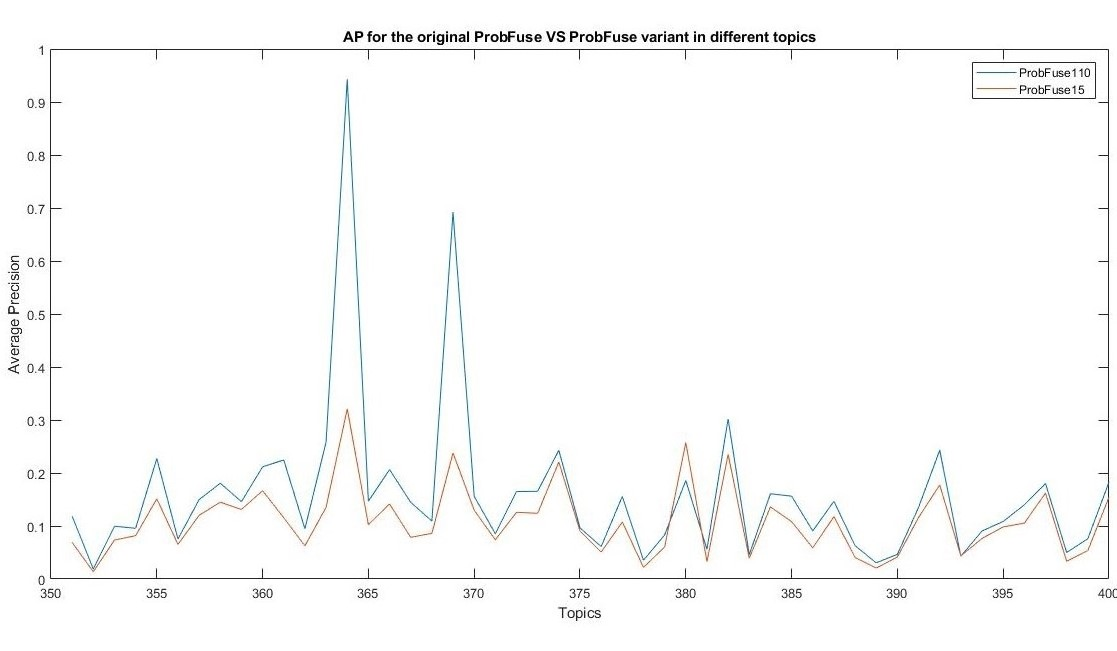
\includegraphics[scale=0.6]{plot3}
\caption{Average Precision for this ProbFuse variant VS the original ProbFuse (with k=110 segments) in different topics}
\label{Average Precision for this ProbFuse variant VS the original ProbFuse (with k=110 segments) in different topics}
\end{figure*}



\textbf{IIX. CONCLUSION}

We have implemented standard rank fusion strategies and ProbFuse algorithm, a data fusion algorithm that relies on the probability of relevance to calculate a ranking score for documents in a fused result set.
These probabilities are calculated based on the position of relevant documents in result sets returned in response to the collection’s queries. For this collection, full relevance judgments were available, so all the document were just been judged. 
By assessing the fused result set given by the different strategies adopted, we have discovered that standard rank fusion strategies are able to achieve results very similar to those obtained through fused result set derived from runs given by different individual models evaluated by Terrier. For some topics, the use of standard strategies has led to achieve results even better than these last. Instead, by comparing fused result set obtained through ProbFuse algorithm and those of standard strategies we have obtained better results for some topics that have been cited previously, for many others topics we have obtained similar results and for about ten topics the results achieved were worse than those derived from standard rank fusion strategies. \\

\end{document}